\section{Deductive synthesis of LTS models from guarded hMSCs}

\begin{frame}{Deductive synthesis of LTS models from guarded hMSCs}

  \begin{block}{Motivation}
    \begin{itemize}
      \item Guarded hMSCs are high-level, intuitive models 
      \begin{itemize}
        \item Concrete syntaxes: directed graph, guarded commands,~\ldots
        \item Structured forms for hMSC and LTS, avoiding state/trace explosion
      \end{itemize}
      \item Trace-based semantics
      \begin{itemize}
        \item Declarative
        \item Ability to reuse/extend available LTS techniques
      \end{itemize}
      \item In practice
      \begin{itemize}
        \item Constructive algorithm to compute the set of admissible traces?
        \item Typically needed for analysis (e.g. model-checking)
      \end{itemize}
    \end{itemize}
  \end{block}

  \begin{block}{Outline}
    \begin{itemize}
      \item From guarded hMSC to guarded LTS
      \item From guarded LTS to pure LTS
      \item Model analysis perspectives of deductive synthesis
    \end{itemize}
  \end{block}

\end{frame}

\subsection{From guarded hMSC to guarded LTS}
\begin{frame}{From guarded hMSC to guarded LTS}

  \begin{center}
    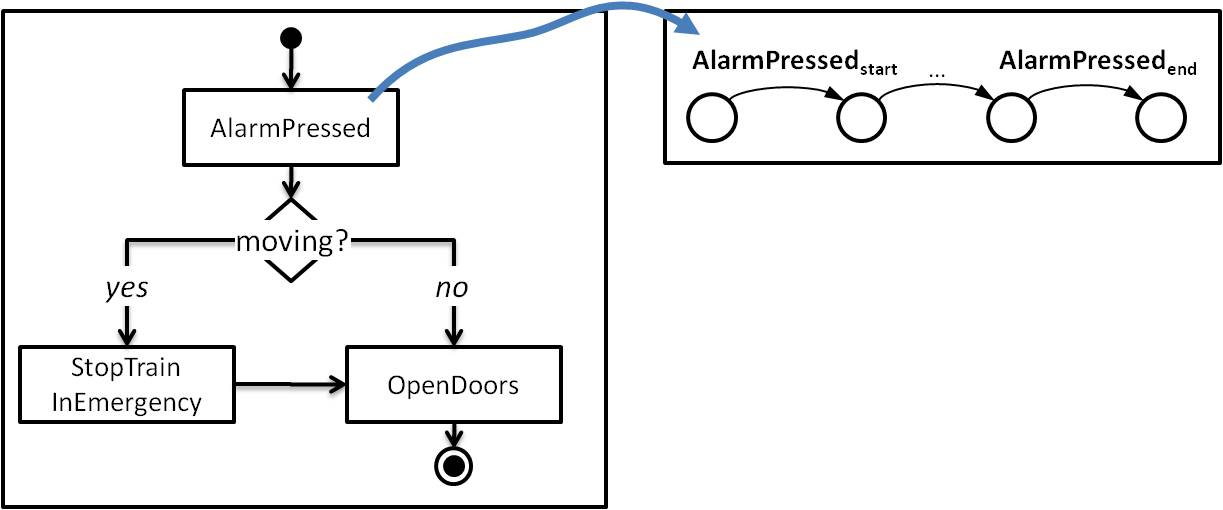
\includegraphics[width=11cm]{images/ghmsc2glts_task.jpg}
  \end{center}
  
  \begin{itemize}
    \item Introduction of $start$ and $end$ events to support more accurate fluent definitions
    \begin{itemize}
      \item refinements yield events between them
    \end{itemize}
  \end{itemize}

\end{frame}


\begin{frame}{From guarded hMSC to guarded LTS}

  \begin{center}
    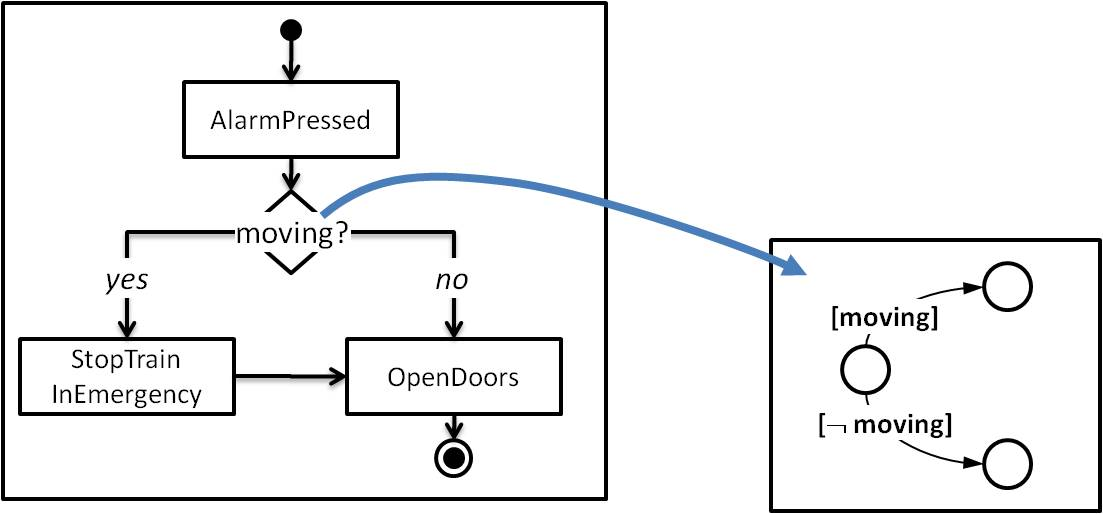
\includegraphics[width=11cm]{images/ghmsc2glts_decision.jpg}
  \end{center}
  
  \begin{itemize}
    \item Decision nodes are converted to guarded transitions
  \end{itemize}

\end{frame}

\begin{frame}{From guarded hMSC to guarded LTS}

  \begin{center}
    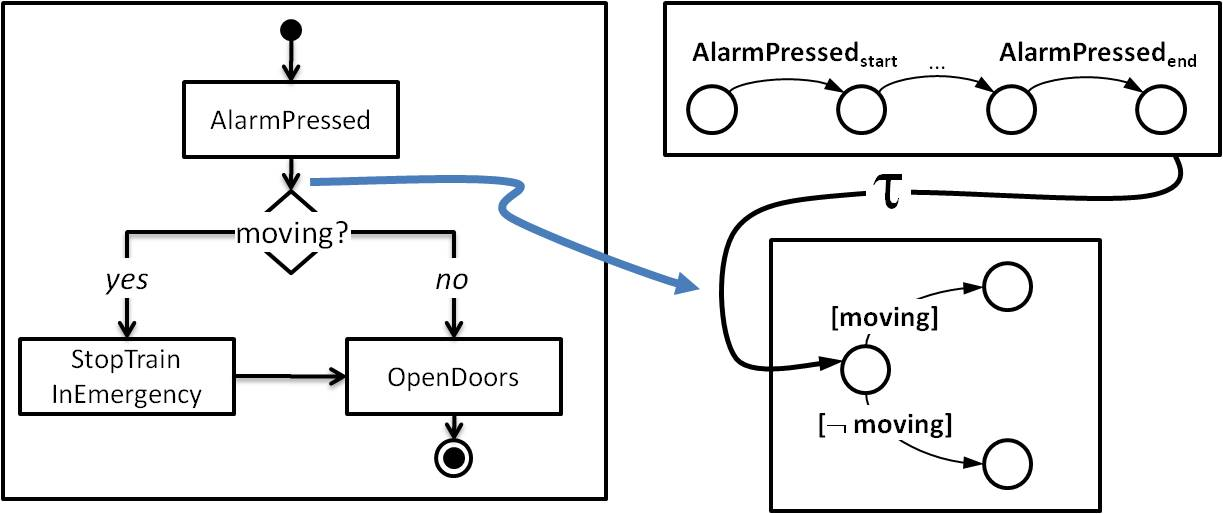
\includegraphics[width=11cm]{images/ghmsc2glts_tau.jpg}
  \end{center}
  
  \begin{itemize}
    \item Bricks connected with $\tau$ transitions
    \begin{itemize}
      \item mapping preserved between g-hMSC and g-LTS (useful for analysis feedback)
    \end{itemize}
  \end{itemize}

\end{frame}

\subsection{From guarded LTS to pure LTS}
\begin{frame}{From guarded LTS to pure LTS}

Algorithm for composing multiple automata

\begin{itemize}
\item Super LTS
  \begin{itemize}
    \item guarded LTS where guards are replaced by special events
    \item to meet the \emph{trace inclusion} condition
  \end{itemize}
\item Initializer LTS
  \begin{itemize}
    \item to meet the \emph{admissible start} condition
  \end{itemize}
\item Fluent automata (one per fluent)
  \begin{itemize}
    \item to meet the \emph{guard satisfaction} condition
  \end{itemize}
\end{itemize}

\end{frame}

\subsection{Model analysis perspectives of deductive synthesis}
\begin{frame}{Model analysis perspectives of deductive synthesis}
\end{frame}
